%----------------------------------------------------------------
%
%  File    :  survey-gtd.tex
%
%  Author  :  Mirza Kabiljagic, Stefan Rajinovic, Aleksandar Stojicic,
%             Inti Gabriel Mendoza Estrada
%
%  Created :  27 May 20xx
%
%  Changed :  05 Dez 2019
%
%----------------------------------------------------------------

\chapter{Good Table Design}
\label{chap:gtd}

We will discuss certain conventions that are widely regarded as ``Good
Table Design''. These conventions are generally neat little CSS tricks
which serve to aesthetically improve the look of a table and in most
cases also add to the effectiveness and efficiency of tables. All tables
must incorporate at least one of the following conventions.


\section{Alternate row highlighting}
When presented a table with a lot of entries, it can be hard to look at.
Scrolling through numerous rows can be frustrating. With this CSS trick,
it can be a bit easier, at least for the eyes, if nothing else. The idea
is to color every even row, while leaving the odd ones intact.
Implementing this techniques requires only two lines of CSS, and is
objectively useful. This can be seen in Listing \ref{AltH}.


\begin{lstlisting}[%
    float=tp,
    language = CSS,
    xleftmargin=0cm,              % no extra margins for floats
    xrightmargin=0cm,             % no extra margins for floats
    language=biblatex,
    basicstyle=\footnotesize\ttfamily,
    frame=shadowbox,
    numbers=left,
    label=list:AltH,
     stringstyle=\color{blue}
    ,
    caption={[Alternate Row Highlighting]
    },
]
% An example of using simple CSS to color table rows:
table.alt tr:nth-child(even) {
  background: #CCC
}

table.alt tr:nth-child(odd) {
  background: #FFF
}
\end{lstlisting}


An example HTML table with this technique is shown in Figure \ref{fig:AltRowHighlight}.
\begin{figure}[tp]
    \centering

    {%
    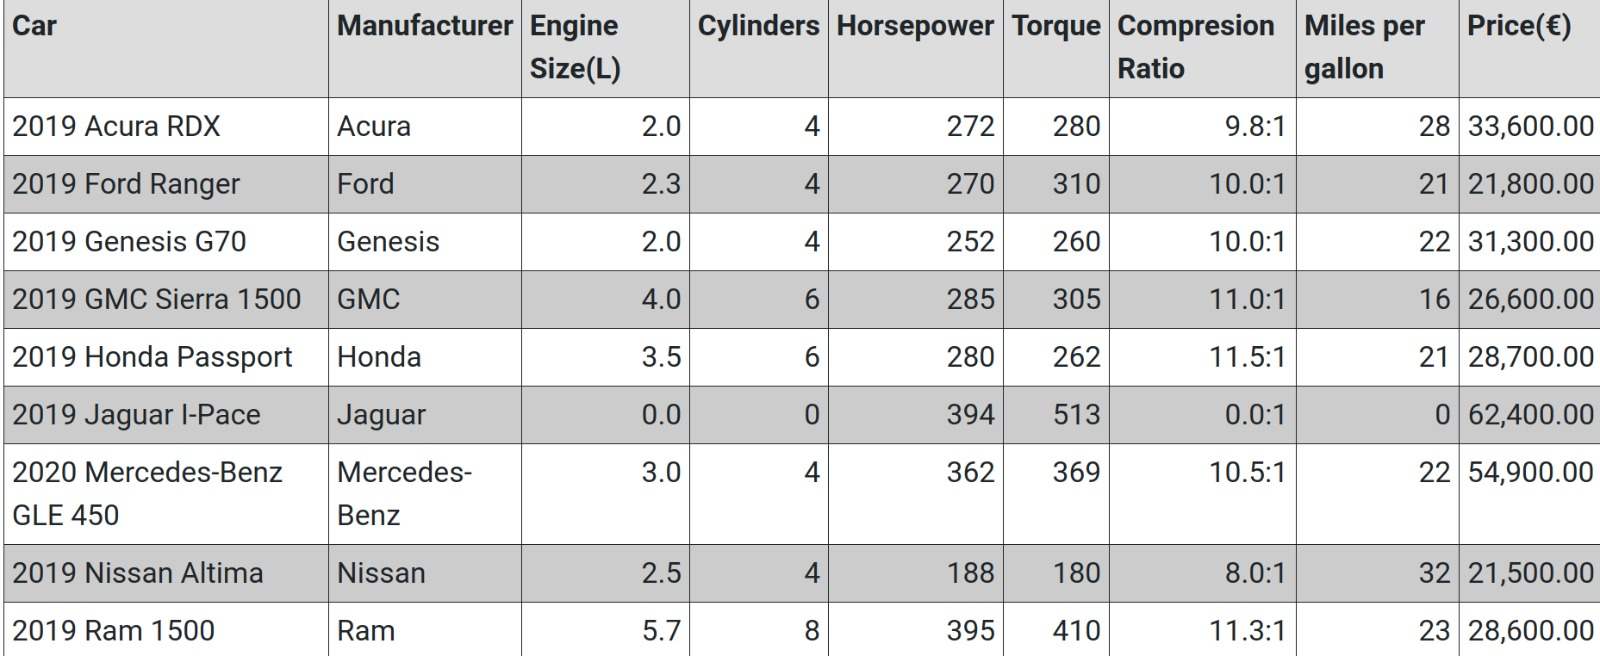
\includegraphics[width=\linewidth]
    {images/alt_t.jpeg}%
    \label{alt_t}%
    }


    \caption[Alternate row highlighting]
    {

    \imgcredit{Screenshot taken by the author.}
    }
    \label{fig:AltRowHighlight}
\end{figure}


\section{Current Row Highlighting}
Just like in Alternate Row Highlighting, `walking' through a big table
one may easily become lost and wouldn't know in which row he is at the
moment, which can be pretty stressful and overall decrease the
efficiency of the table. 

With the help of some CSS, the lives of the users are made easier. This code can be seen
in Listing \ref{list:CurrentRow}

\begin{lstlisting}[%
    language = HTML,
    xleftmargin=0cm,              % no extra margins for floats
    xrightmargin=0cm,             % no extra margins for floats
    language=biblatex,
    basicstyle=\footnotesize\ttfamily,
    frame=shadowbox,
    numbers=left,
    label=list:CurrentRow,
     stringstyle=\color{blue}
    ,
    caption={[Current Row Highlighting]
    },
]
% An example of using simple CSS to highlight table rows:
table {
  overflow: hidden;
}

tr:hover {
  background-color: #ffa;
}

td, th {
  position: relative;
}

td:hover::after, th:hover::after {
  content: "";
  position: absolute;
  background-color: #ffa;
  left: 0;
  width: 100%;
  z-index: -1;
}
\end{lstlisting}


An example HTML table with this technique is shown in Figure \ref{fig:CurrentRowHighlight}.
\begin{figure}[tp]
    \centering

    {%
    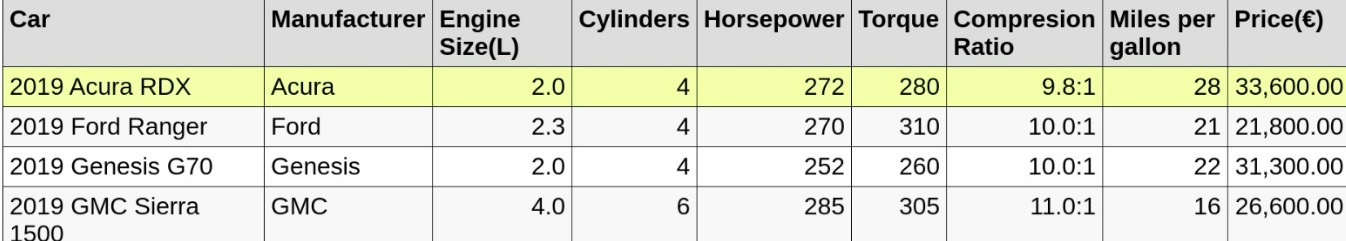
\includegraphics[width=\linewidth]
    {images/current_hl.jpeg}%
    \label{current_hl}%
    }


    \caption[Current Row Highlighting]
    {

    \imgcredit{Screenshot taken by the author.}
    }
    \label{fig:CurrentRowHighlight}
\end{figure}

\section{Expandable Areas}
Should we have any further information available about a table's object,
making the row clickable and showing the extra information is a better
alternative than trying to cram everything inside the table. In the
code snippet shown in Listing \ref{list:ExpArea} we see how additional data in 
an HTML table can be implemented \parencite{Alligator}.

\begin{lstlisting}[%
    float = tp,
    language = CSS,
    xleftmargin=0cm,              % no extra margins for floats
    xrightmargin=0cm,             % no extra margins for floats
    language=biblatex,
    basicstyle=\footnotesize\ttfamily,
    frame=shadowbox,
    numbers=left,
    label=list:ExpArea,
     stringstyle=\color{blue}
    ,
    caption={[Expandable Area Before]
    },
]
<tr>
  <td>2019 Acura RDX</td>
  <td>Acura</td>
  <td style="text-align: right">2.0</td>
  <td style="text-align: right">4</td>
  <td style="text-align: right">272</td>
  <td style="text-align: right">280</td>
  <td style="text-align: right">9.8:1</td>
  <td style="text-align: right">28</td>
  <td style="text-align: right">33,600.00</td>
</tr>
<tr>
  <td colspan="5">
    <h4>Additional information about the car</h4>

    <ul>
      <li><a href="https://en.wikipedia.org/wiki/Acura_RDX">Acura RDX</a>
      </li>
      <li><a href="https://www.acura.ca/rdx">Acura RDX official webpage</a>
      </li>
    </ul>
  </td>
</tr>
<tr>
\end{lstlisting}
To implement this table feature the combination of JavaScript and CSS
needs to be implemented. In the snippet codes in Listings \ref{list:ExpArea2} and \ref{list:ExpArea3}, the JavaScript and
CSS code can be reviewed.

\begin{lstlisting}[%
    language = HTML,
    xleftmargin=0cm,              % no extra margins for floats
    xrightmargin=0cm,             % no extra margins for floats
    language=biblatex,
    basicstyle=\footnotesize\ttfamily,
    frame=shadowbox,
    numbers=left,
    label=list:ExpArea2,
     stringstyle=\color{blue}
    ,
    caption={[Expandable Area After]
    },
]
<script type="text/javascript">
$(document).ready(function(){

  $("#report tr:odd").addClass("odd");
  $("#report tr:not(.odd)").hide();
  $("#report tr:first-child").show();

  $("#report tr.odd").click(function () {
    var trToToggle = $(this).next("tr");
    $("#report tr:not(.odd)").not(trToToggle).hide();
    $("#report tr:first-child").show();
    $(trToToggle).toggle();
    $(this).find(".arrow").toggleClass("up");
  });
})
</script>

\end{lstlisting}

\begin{lstlisting}[%
    float = tp,
    language = CSS,
    xleftmargin=0cm,              % no extra margins for floats
    xrightmargin=0cm,             % no extra margins for floats
    language=biblatex,
    basicstyle=\footnotesize\ttfamily,
    frame=shadowbox,
    numbers=left,
    label=list:ExpArea3,
     stringstyle=\color{blue}
    ,
    caption={[Expandable Area ]
    },
]
#report {
  border-collapse:collapse;
}
#report h4 {
  margin:0rem;
  padding:0rem;
}
#report img {
  float:right;
}
#report ul {
  margin:0.625rem 0 0.625rem 2.5rem;
  padding:0rem;
}
#report th {
  background:#7CB8E2  repeat-x scroll center left;
  color:#fff;
  padding:0.4375rem 0.9375rem;
  text-align:left;
}
#report td {
  background:#C7DDEE none repeat-x scroll center left;
  color:#000;
  padding:0.4375rem 0.9375rem;
}
#report tr.odd td {
  cursor:pointer;
}
#report div.arrow {
  background:transparent url(arrows.png) no-repeat scroll 0rem -1rem;
  width:1rem;
  height:1rem;
  display:block;
}
#report div.up {
  background-position:0rem 0rem;
}
\end{lstlisting}

An example HTML table with this technique before a row is clicked is 
shown in Figure \ref{fig:ExpandArea}.
\begin{figure}[tp]
    \centering

    {%
    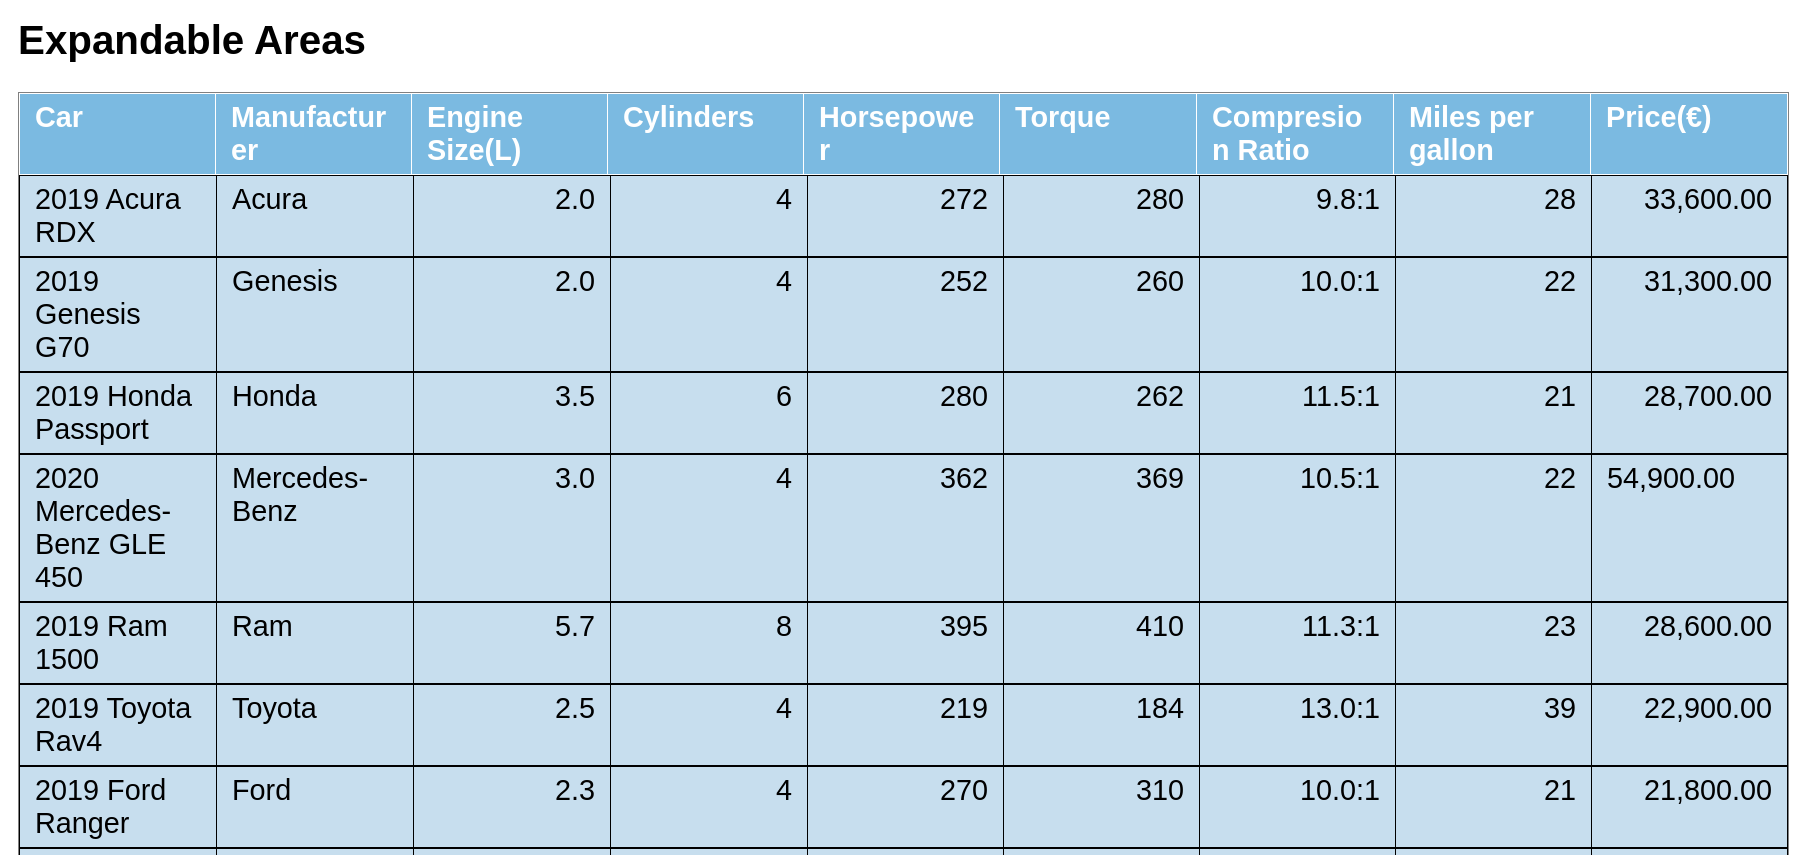
\includegraphics[width=\linewidth]
    {images/expandable_area_before.png}%
    \label{exp_area_before}%
    }


    \caption[Expandable Areas]
    {

    \imgcredit{Screenshot taken by the author.}
    }
    \label{fig:ExpandArea}
\end{figure}

An example HTML table with this technique after a row is clicked is 
shown in Figure \ref{fig:exp_areas}.
\begin{figure}[tp]
    \centering

    {%
    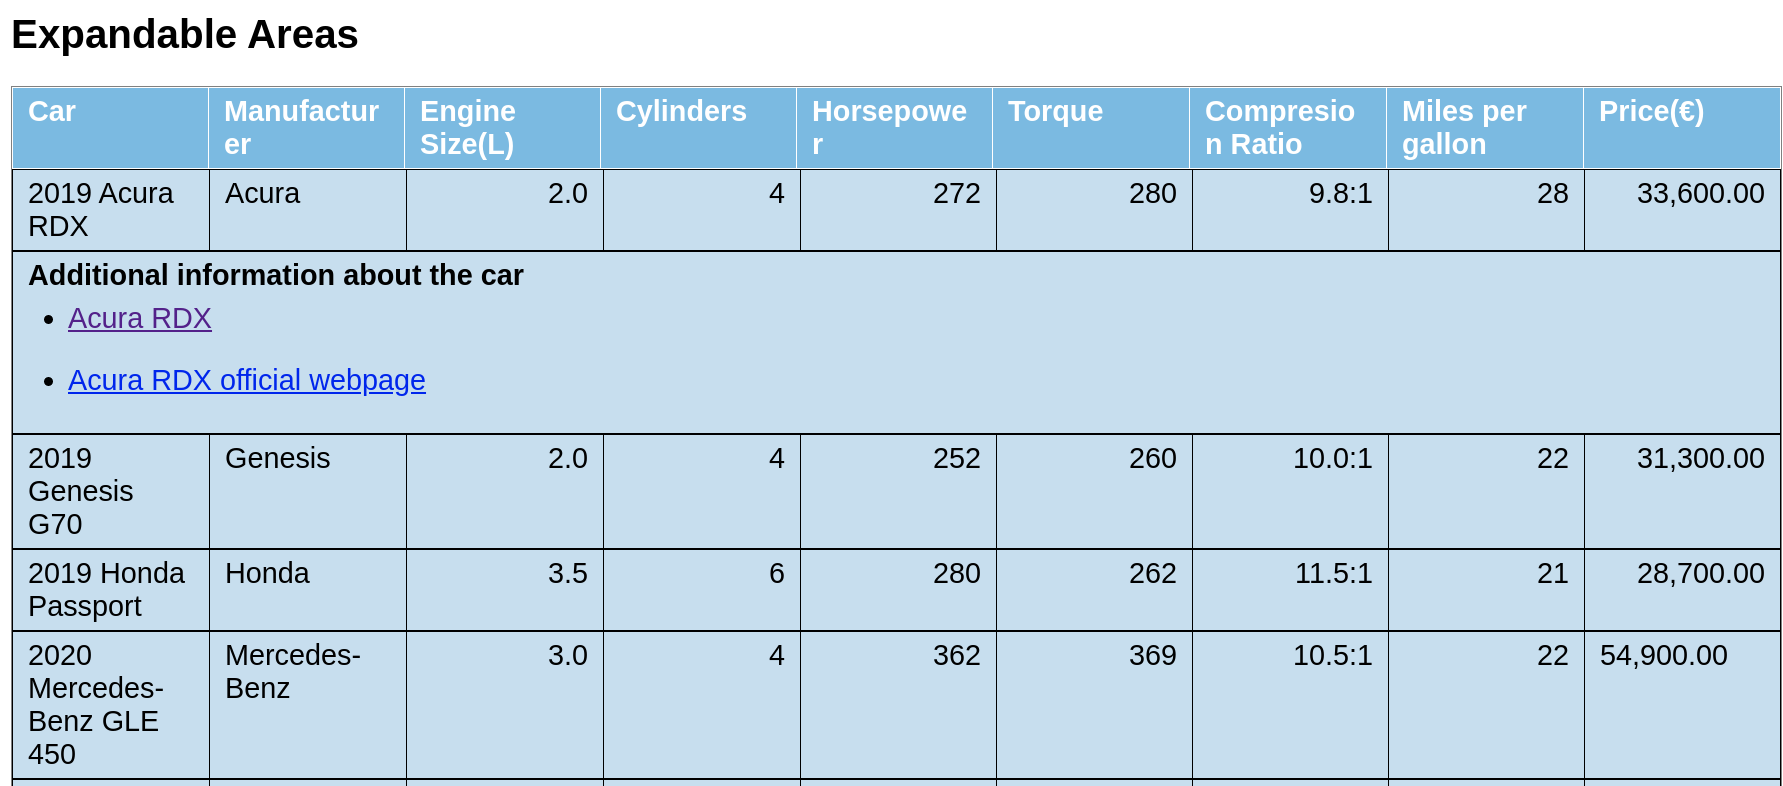
\includegraphics[width=\linewidth]
    {images/expandable_areas_after.png}%
    \label{exp_area_after}%
    }


    \caption[Expandable Areas]
    {

    \imgcredit{Screenshot taken by the author.}
    }
    \label{fig:exp_areas}
\end{figure}

\section{Pagination (With Sort and Search)}
The amount of data increases every second, over 2.5 quintillion bytes of
 data are made every day and there is also estimation that in 2020 will
 be created 1.7MB of data in every second for each person in the
 world\parencite{PG_2}. Tables are one of the best mediums for displaying large sets of data
efficiently. Features can be added to tables to increase efficiency even
more. For example, if a table is too long, it can be divided into
`pages'. Each page houses a certain amount of rows. The user then can
`flip' through these pages as page navigation is also implemented.

Furthermore, it is possible to sort the table by column (in
ascending/descending and alphabetical order), and search for an element
in the table. This solution works for following browsers:
\begin{itemize}
    \item[--] Google Chrome
    \item[--] Mozzila Firefox
    \item[--] Internet Explorer
    \item[--] Opera
    \item[--] Microsoft Edge
\end{itemize}

For the implementation plug-in for the jQuery Javascript library called 
DataTables is used \parencite{PG_1}. This can be seen in Listing \ref{list:Pagination}.


\begin{lstlisting}[%
  language = CSS,
  xleftmargin=0cm,              % no extra margins for floats
  xrightmargin=0cm,             % no extra margins for floats
  language=biblatex,
  basicstyle=\footnotesize\ttfamily,
  frame=shadowbox,
  numbers=left,
  label=list:Pagination,
  stringstyle=\color{blue}
  ,
  caption={[Pagination ]
    },
]
% An example of using Javascript plugin DataTable():
%Include these two files in order to include additional advanced features to any HTML table
%cdn.datatables.net/1.10.20/css/jquery.dataTables.min.css
%cdn.datatables.net/1.10.20/js/jquery.dataTables.min.js
$(document).ready(function(){
    $('#myTable').dataTable(); //this plugin provides searching, sorting and pagination
 });

\end{lstlisting}

Table is initilaized with "myTable" id and this id is used in ready
 function() to assign dataTable funcionality to our HTML table
 instance\parencite{PG}. An example HTML table with this technique when using the sort feature on
the \propname{Price} column is shown in Figure \ref{fig:pagination_with_sort}
\begin{figure}[tp]
    \centering

    {%
    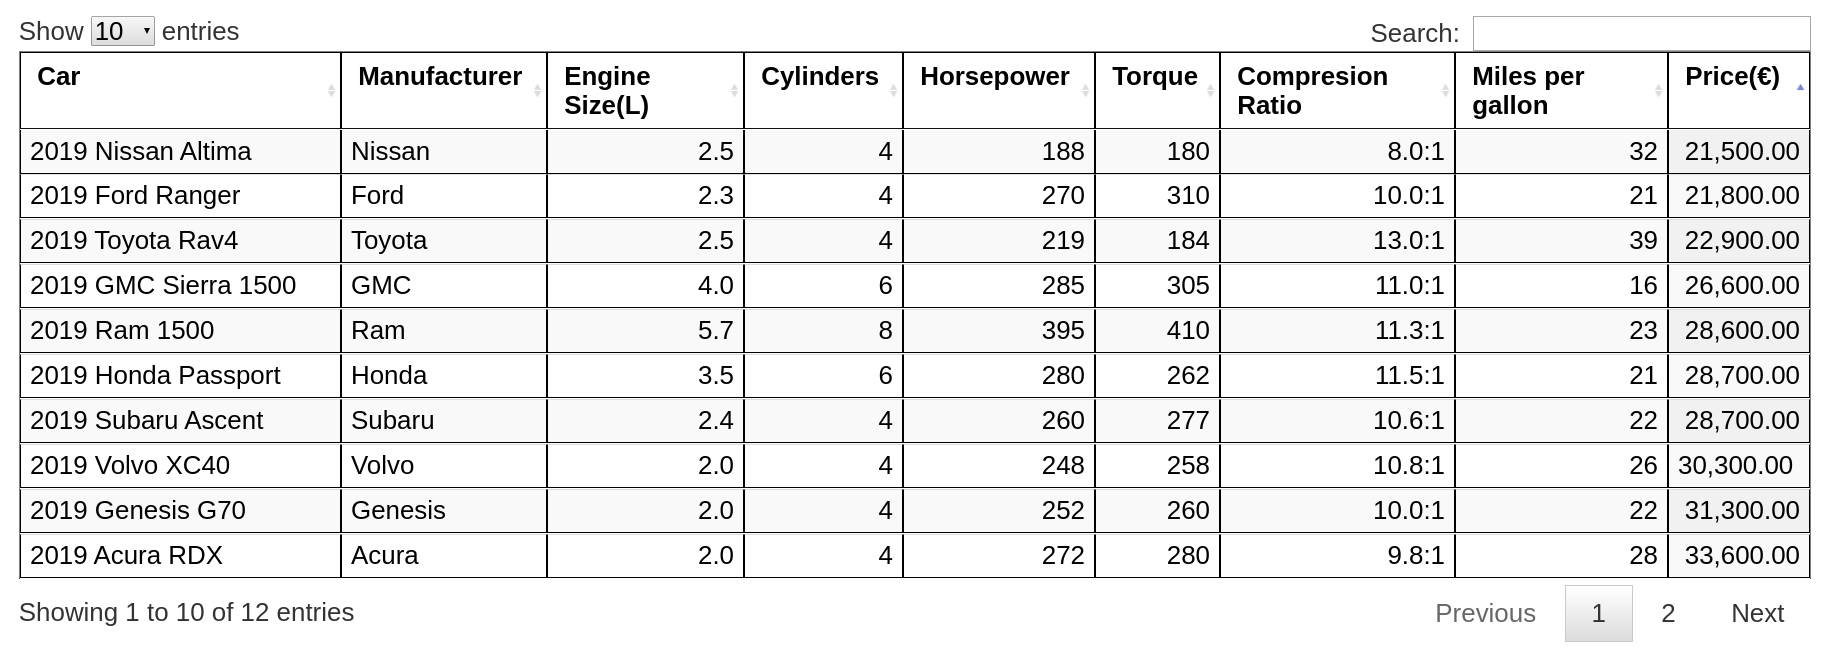
\includegraphics[width=\linewidth]
    {images/pagination_2.png}%
    \label{pagination_2}%
    }


    \caption[Pagination with sort option]
    {

    \imgcredit{Screenshot taken by the author.}
    }
    \label{fig:pagination_with_sort}
\end{figure}

An example HTML table with this technique when using the search feature
is shown in Figure \ref{fig:pagination_with_search}.
\begin{figure}[tp]
    \centering

    {%
    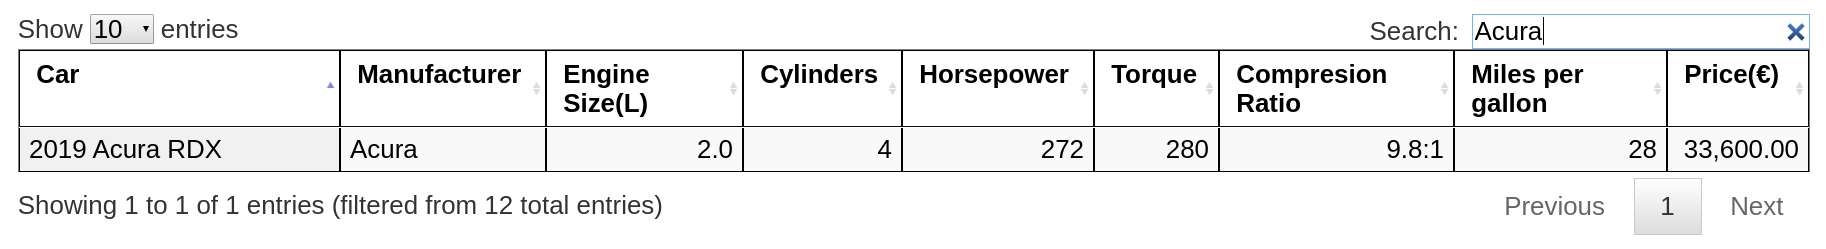
\includegraphics[width=\linewidth]
    {images/pagination_1.png}%
    \label{pagination_1}%
    }


    \caption[Pagination with search option]
    {

    \imgcredit{Screenshot taken by the author.}
    }
    \label{fig:pagination_with_search}
\end{figure}

